\begin{itemize}
	%\item mention/explain TEAMPLAY \texttt{blocks}, \texttt{blockenergy},
    %      \texttt{blocktime}, etc?
	%\item \sout{\texttt{Eq} was already implemented (using `native' things)}
    %      \texttt{NEq} was more complicated (different ways \texttt{Nat}s can be
    %	  not equal)
    %\item explain how only \texttt{LTE} is required for that selection of
    %	  operators?
    %   \item \textbf{explain the structure of operators and decidability rules}
    %\item \texttt{And} was already implemented with custom types, used this as
    %	  inspiration for implementation of \texttt{Or}
    \item explain how these `building blocks'/operators go together (similar to
    	  a stack-based language)?
\end{itemize}

The first section (\ref{des:tp-dsl}) focuses on describing existing work done by the \textsc{TeamPlay} project \cite{teamplay:d1.1}. The remaining sections (\ref{des:neq}, \ref{des:or}, and \ref{des:not}) describe extensions of the \textsc{TeamPlay} system, implemented by me.


\section{The TeamPlay Project}\label{des:tp-dsl}
    \subsection{Assertions and Contracts}
        \begin{figure}[H]
            \centering
            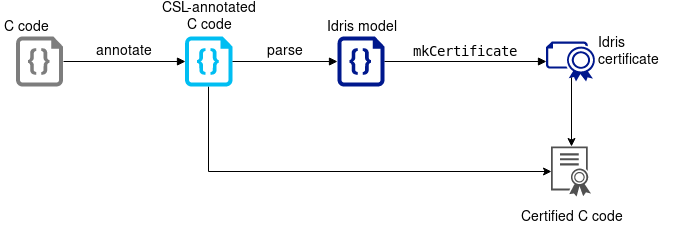
\includegraphics[width=\textwidth]{diagrams/process.png}
            \caption{The process of creating a certified C program}
        \end{figure}
        When writing C programs for embedded systems, the programmer might want to capture extra-functional properties like the time taken or the energy consumed. Furthermore, the programmer may want to have provable guarantees that these properties of the program hold. This is done through contracts which can be proven using the \Idris proof system. The Contract Specification Language (CSL) defined by the \textsc{TeamPlay} project \cite{teamplay:d1.1} lets the programmer annotate existing C code to express properties like the worst time cost of a loop or function, using \texttt{\_\_teamplay\_worst\_time}, and assert these, using \texttt{\_\_teamplay\_assert}. This results in a program whose extra-functional properties can be certified to hold. Since the CSL functions adhere to the C99 function naming scheme, the programmer does not need to change tools, libraries, compiler, or learn a new language. Instead, the annotations seamlessly integrate with the existing code, without disturbing its operation in any way. Once the code has been annotated, it can then be passed through a C parser which extracts the annotations and constructs a model in an \Idris-based DSL. This model is then passed through the \texttt{mkCertificate} function which constructs a contract/certificate specifying which properties do or do not hold, by using the \Idris proof system.
        \begin{table}
            \centering
            \begin{tabular}{c | c}
                \textbf{C operator} & \Idris-based \textbf{DSL equivalent}   \\
                \hline
                \texttt{==}         & \texttt{Eq}     \\
                \texttt{!=}         & \texttt{NEq}    \\
                \texttt{<=}         & \texttt{LTE}    \\
                \texttt{<}          & \texttt{LT}     \\
                \texttt{>=}         & \texttt{GTE}    \\
                \texttt{>}          & \texttt{GT}     \\
                \texttt{\&\&}       & \texttt{And}    \\
                \texttt{||}         & \texttt{Or}     \\
                \texttt{!}          & \texttt{Not}
            \end{tabular}
            \caption{C to DSL mappings}
        \end{table}
    
        \begin{code}[label={des:assertion}, caption={The \texttt{Assertion} data type}]
            data Assertion  : Type where
                MkAssertion : BooleanExpression -> Assertion
        \end{code}
    
        Contracts/Certificates consists of one or more \texttt{Assertion}.
        These are created through the \texttt{MkAssertion} constructor. It takes a \texttt{BooleanExpression} and returns an \texttt{Assertion} based on it. \texttt{BooleanExpression}s are created by applying operators to \texttt{NumericExpression}s or existing \texttt{BooleanExpression}s.
    
    \newpage
    
    \subsection{Numeric Operators and Numeric Expressions}
        The numeric operators all take two arguments, their evaluation, a proof concerning what the operator evaluates to, and returns a \texttt{BooleanExpression}.
        The operands are \texttt{NumericExpression}s. A \texttt{NumericExpression} is defined by the following grammar:
        \setlength{\grammarindent}{12em}
        \begin{grammar}
            <NumericExpression>
            ::=  ; a literal\\
                 `Lit' <digit>$^+$
            \alt ; a variable\\
                 `Var' <identifier>
            \alt ; a parenthesised expression\\
                 `NParen' <NumericExpression>
            \alt ; addition\\
                 `Plus' <NumericExpression> <NumericExpression>
            \alt ; subtraction\\
                 `Sub' <NumericExpression> <NumericExpression>
            \alt ; multiplication\\
                 `Mul' <NumericExpression> <NumericExpression>
            \alt ; division\\
                 `Div' <NumericExpression> <NumericExpression>
            \alt ; modulo\\
                 `Mod' <NumericExpression> <NumericExpression>
        \end{grammar}
        \texttt{NumericExpression}s are evaluated given an environment \texttt{Env}. The environment is essentially a mapping from symbols to values.
        \begin{code}[caption={The type of the \texttt{eval} function}]
            eval : Env -> NumericExpression -> Nat
        \end{code}
        The \texttt{eval} function uses this to evaluate a \texttt{NumericExpression}: Given an \texttt{Env} and a \texttt{NumericExpression}, the \texttt{eval} function returns a natural number. This is the result of that \texttt{NumericExpression} over that environment. To use the evaluation in a proof, we use the \texttt{Evald} type.
        \begin{code}[caption={\texttt{Evald} as defined in the \Idris model},label={des:evald}]
    data Evald : NumericExpression -> Nat -> Type where
        MkEvald : (x : NumericExpression) -> (y : Nat) -> Evald x y
        \end{code}
        Listing \ref{des:evald} shows that \texttt{Evald} is a data type constructed from a \texttt{NumericExpression} and \texttt{Nat}. This  is because \texttt{eval} only evaluates the expression, it does not provide a proof linking the evaluated value and the original expression. The \texttt{Evald} type `links' the numeric expression (\texttt{x}) and its evaluation (\texttt{y}), proving that \texttt{x} evaluates to \texttt{y}.
        \\
        
        When applying a numeric operator to some \texttt{NumericExpression}s, we get a \texttt{BooleanExpression}.
    
    \subsection{Boolean Operators and Boolean Expressions}
        Boolean expressions result from either a numeric operator or a boolean operator. The grammar for constructing boolean expressions is:
        \setlength{\grammarindent}{11em}
        \begin{grammar}
            <BooleanExpression>
            ::=  ; a paranthesised expression\\
            `BParen' <BooleanExpression>
            \alt ; the negation of an expression\\
            `Not' <BooleanExpression>
            \alt ; the conjunction of two expressions\\
            `And' <BooleanExpression> <BooleanExpression>
            \alt ; the disjunction of two expressions\\
            `Or' <BooleanExpression> <BooleanExpression>
            \alt ; testing two numbers for equality\\
            `Eq' <NumericExpression> <NumericExpression>
            \alt ; testing two numbers for inequality\\
            `NEq' <NumericExpression> <NumericExpression>
            \alt ; whether one number is strictly less than the other\\
            `LT' <NumericExpression> <NumericExpression>
            \alt ; whether one number is less than or equal to the other\\
            `LTE' <NumericExpression> <NumericExpression>
            \alt ; whether one number is strictly greater than the other\\
            `GT' <NumericExpression> <NumericExpression>
            \alt ; whether one number is greater than or equal to the other\\
            `GTE' <NumericExpression> <NumericExpression>
        \end{grammar}
        Similar to \texttt{NumericExpressions}, \texttt{BooleanExpressions} are evaluated over an environment.
        \begin{code}[caption={The type of the \texttt{beval} function}]
            beval : Env -> BooleanExpression -> Bool
        \end{code}
        Given an \texttt{Env} and a \texttt{BooleanExpression}, the \texttt{beval} function returns a boolean. This boolean is the result of evaluating that \texttt{BooleanExpression} over that environment. Like with \texttt{NumericExpressions}, to use the evaluation in a proof, we have the \texttt{BEvald} type.
        \begin{code}[caption={\texttt{BEvald} as defined in the \Idris model}]
data BEvald : BooleanExpression -> Nat -> Type where
    MkBEvald : (x : BooleanExpression) -> (y : Bool) -> BEvald x y
        \end{code}
        \texttt{BEvald} works like \texttt{Evald} except for boolean expressions and values. It is a data type constructed from a \texttt{BooleanExpression} and a \texttt{Bool}. Like \texttt{eval}, the \texttt{beval} function only evaluates the value of the boolean expression, it does not provide a proof that the expression evaluates to that boolean. The \texttt{BEval} type is a proof that the boolean expression \texttt{x} evaluates to the boolean \texttt{y}.
        
    \subsection{The \texttt{LTE} operator}\label{des:tp:lte}
        The less-than-or-equals operator, \texttt{LTE}, is the only operator defined in the \Idris prelude, as the other similar operators (i.e. \texttt{LT}, \texttt{GTE}, and \texttt{GT}) can be defined from it.
        
        \begin{code}[caption={\texttt{LT} can be defined based on \texttt{LTE}}]
        isLT : (m : Nat) -> (n : Nat) -> Dec (LTE (S m) n)
        isLT m n = isLTE (S m) n
        \end{code}
        
        Strictly less-than, \texttt{LT}, can be defined from less-than-or-equals as follows: if the successor of a number $m$ is LTE to another number $n$, then $m$ is strictly less-than $n$; $(m + 1) \leq n \Rightarrow m < n$.
        
        \begin{code}[caption={\texttt{GTE} can be defined based on \texttt{LTE}}]
        isGTE : (m : Nat) -> (n : Nat) -> Dec (LTE n m)
        isGTE m n = isLTE n m
        \end{code}
        
        Greater-than-or-equals, \texttt{GTE}, can be defined from less-than-or-equals by simply swapping the operands: if a number $n$ is LTE to a number $m$ then $m$ is greater-than-or-equal to $n$; $n \leq m \Rightarrow m \geq n$.
        
        \begin{code}[caption={\texttt{GT} can be defined based on \texttt{LTE}}]
        isLT : (m : Nat) -> (n : Nat) -> Dec (LTE (S n) m)
        isLT m n = isLTE (S n) m
        \end{code}
        
        Finally, strictly greater-than, \texttt{GT}, can be defined as a `combination' of the definitions of \texttt{LT} and \texttt{GTE}: if the successor of a number $n$ is LTE to a number $m$ then $m$ is strictly greater-than to $n$; $(n + 1) \leq m \Rightarrow m > n$.
        \\
        
        The operators \texttt{And}, \texttt{Eq}, \texttt{LT}, \texttt{LTE}, \texttt{GT}, and \texttt{GTE} were already implemented. In order to have a complete set of operators, I implemented \texttt{NEq}, \texttt{Or}, and \texttt{Not}.


\section{Inequality (\texttt{NEq})}\label{des:neq}
    \texttt{Eq} had already been implemented by the \textsc{TeamPlay} project, using the built-in \texttt{(=)} data type and the \texttt{DecEq} interface, as part of the D1.1 deliverable \cite{teamplay:d1.1}.
    
    \subsection{The \texttt{(=)} data type}
        \begin{code}[label={des:refl-concept}, caption={The concept of an equality data type}]
        data (=) : a -> b -> Type where
            Refl : x = x
        \end{code}
    
        A very useful pre-defined data type is the \texttt{(=)} data type. It is not quite defined as a data type since `\texttt{=}' is a reserved symbol, instead it is part of the \Idris syntax. It is still a data type, just defined at a lower level of the language than the \texttt{data} construct. Its constructor \texttt{Refl} is short for `reflexive'. Reflexivity is a mathematical concept stating that every element in a set is related to itself. In logic, one would write $\forall x \in X : x R x$ where $X$ is a set of elements $x$ and $R$ is a binary relation. This further means that \texttt{=} also must be symmetric and transitive: if $x = y$ then $y = x$; and if $x = y$ and $y = z$ then $x = z$. In short, if two elements are reflexive, this means they are the same element. \textbf{[correct?]}
    
        \begin{code}[label={des:refl-egs}, caption={Examples of reflexivity}]
        Idris> the ("World" = "World") Refl
        Refl : "World" = "World"
        
        
        Idris> the (True = True) Refl
        Refl : True = True
        
        
        Idris> the (1 + 2 + 3 = 6) Refl
        Refl : 6 = 6
        \end{code}
        At the \Idris prompt, we can use the \texttt{the} function to create some example instances of \texttt{Refl}. The last example shows that \Idris evaluates the sides of a type before trying to construct the \texttt{Refl}.
    
        \newpage
    
        \begin{code}[label={des:not-refl}, caption={Things that are not reflexive}, escapeinside={(*}{*)}]
        Idris> the ("Foo" = "Bar") Refl
        (input):1:1-24:When checking argument value to function
        Prelude.Basics.the:
            Type mismatch between
                x = x (Type of Refl)
            and
                "Foo" = "Bar" (Expected type)
        
            Specifically:
                Type mismatch between
                    "Foo"
                and
                    "Bar"
        
        
        Idris> the (True = False) Refl
        (input):1:1-23:When checking argument value to function
        Prelude.Basics.the:
            Type mismatch between
                x = x (Type of Refl)
            and
                True = False (Expected type)
        
            Specifically:
                Type mismatch between
                    True
                and
                    False
        
        
        Idris> the (2 = 3) Refl
        (input):1:1-16:When checking argument value to function
        Prelude.Basics.the:
            Type mismatch between
                3 = 3 (Type of Refl)
            and
                2 = 3 (Expected type)
            
            Specifically:
                Type mismatch between
                    3
                and
                    2
        \end{code}
        If we try to instantiate \texttt{Refl} using elements which are not reflexive, the type-checker complains and tells us that it does not make sense and so we cannot create a \texttt{Refl} from things which are not reflexive. The \texttt{Refl} type can be used to prove that things are equal, since it can only exist if the things truly are equal. In order to prove the opposite, that things cannot be equal, we use a different data type.
    
    \subsection{The \texttt{TyNEq} data type}
        Because there is no built-in \texttt{NEq} data type, I had to define one.
        \begin{code}[label={des:neq:ty-neq}, caption={The data type used for capturing inequality}]
        data TyNEq : Nat -> Nat -> Type where
            MkNEqL   : TyNEq Z (S k)
            MkNEqR   : TyNEq (S k) Z
            MkNEqRec : TyNEq k j -> TyNEq (S k) (S j)
        \end{code}
        The constructors for the \texttt{TyNEq} data type describe the different ways numbers can be not equal:
        \begin{itemize}
            \item \textbf{The first number is zero and the second is not} -- in this case the numbers are not equal, specifically the left number is zero. Since no number can have zero as its successor, the numbers are not equal.
            \item \textbf{The second number is zero and the first is not} -- in this case, the numbers are not equal, specifically the right number is zero. Since no number can have zero as its successor, the numbers are not equal.
            \item \textbf{The numbers are not equal} -- in this case, the successors of the numbers must also be not equal. For example, $2 \neq 5 \rightarrow 3 \neq 6 \rightarrow 4 \neq 7$ etc.
        \end{itemize}
        Using the \texttt{TyNEq} data type, we can then define \texttt{NEq}.
        \begin{code}[label={des:neq-code}, caption={The definition of \texttt{NEq}}, escapeinside={(*}{*)}]
        data BooleanExprssion : Type where
            (*\vdots*)
            
            NEq :  (x : NumericExpression)
                -> (y : NumericExpression)
                -> Evald x x'
                -> Evald y y'
                -> Dec (TyNEq x' y')
                -> BooleanExpression
            (*\vdots*)
        \end{code}
    
        \texttt{NEq} takes two numeric expressions, proofs of what they evaluate to, and a decidable proof of whether the numeric expressions are inequal. From this, \texttt{NEq} returns a \texttt{BooleanExpression} which will evaluate to \texttt{True} if the numeric expressions were not equal, and \texttt{False} otherwise. For the decidability part,\linebreak
        \texttt{Dec (TyNEq x' y')}, we need some proof functions which either prove that two numbers must be unequal or prove that they cannot possibly be.
    
    \subsection{The \texttt{Void} data type and the \texttt{void} function}
        The \Idris prelude has a `\texttt{Void}' data type. It expresses the impossibility of something happening.
    
        \begin{code}[caption={The \texttt{Void} type has no constructors}]
        data Void : type where
        \end{code}
        Since \texttt{Void} has no constructors, it is impossible to directly create an instance of \texttt{Void}. Therefore, if a function returns an instance of \texttt{Void}, this means that its arguments resulted in something which is impossible to create. From a logical point of view, the arguments to the function express a contradiction, and as such \texttt{Void} represents something which can only be constructed if we accept that the contradiction is true.
        
        \begin{code}[label={idr:zns}, caption={Zero cannot be the successor of a natural number}]
        zeroNotSuc : (0 = S k) -> Void
        zeroNotSuc Refl impossible
        \end{code}

        The first argument to the \texttt{zeroNotSuc} function is a reflexive equality expressing that zero is the successor of some natural number \texttt{k}. This is impossible and as such we cannot construct the \texttt{Refl}, which means that the function could return a \texttt{Void}. The `\texttt{impossible}' keyword tells the \Idris type checker that the pattern must not type check. Since we could not possibly have a \texttt{Refl : 0 = S k}, this holds.
        
        \newpage
        
        \begin{code}[caption={Invalid use of the \texttt{impossible} keyword}, escapeinside={(*}{*)}]
        boolRefl : (b : Bool) -> (b = b)
        boolRefl True = Refl
        boolRefl False impossible
        
        
        (*\underline{\textnormal {Compiler error:}}*)
        
          |
        3 | boolRefl False impossible
          |                ~~~~~~~~~~
        boolRefl False is a valid case
        \end{code}
        The \texttt{boolRefl} function here simply shows that booleans are reflexive. If we try to use the \texttt{impossible} keyword for the \texttt{False} case, the type checker complains and tells us that it \textit{is} a valid case.
        
        \begin{code}[label={idr:snz}, caption={The successor of a natural number cannot be zero}]
        sucNotZero : (S k = 0) -> Void
        sucNotZero Refl impossible
        \end{code}
        Similar to stating that zero cannot be the successor of a number, we can state that no natural number \texttt{k} can have zero as its successor. If we could create a\linebreak
        \texttt{Refl : S k = 0}, we could create an instance of \texttt{Void}. Actually, if we could create an instance of \texttt{Void}, we would be able to create an instance of any type. Or logically: if we accept a contradiction to be true, we can prove anything.
    
    
        \begin{code}[caption={The \texttt{void} function}]
        void : Void -> a
        \end{code}
    
        The pre-defined \texttt{void} function captures this: given an instance of \texttt{Void}, the \texttt{void} function returns an instance of any type. This may seem like a peculiar thing to have: a function whose input cannot exist. However, if we can say that certain things \textit{cannot} happen, we can use that to say more precisely what \textit{can} happen.
        
        \begin{code}[label={des:no-rec}, caption={Applying a function to an impossibility does not make it possible}]
        noRec : (contra : (k = j) -> Void) -> (S k = S j) -> Void
        noRec contra Refl = contra Refl
        \end{code}
        
        The \texttt{noRec} function takes a proof that two natural numbers are not equal and proves that their successors must then also be not equal. Given a \texttt{contra} which is a function from \texttt{(k = j)} to \texttt{Void} and a \texttt{Refl} representing\linebreak
        \texttt{(S k = S j)}, we can use the \texttt{contra} function to return an instance of \texttt{Void}. Hence, the
        \texttt{Refl : S k = S j} cannot exist.
    
    \subsection{Decidability}
        Decidability is more specific than \texttt{Maybe}. Instead of saying that we have \texttt{Just} the value or \texttt{Nothing}, decidability allows us to express that we can always \textit{decide} whether a property holds or not for certain values.
    
        \begin{code}[caption={\texttt{Dec} as defined in the \Idris prelude}]
        data Dec : (prop : Type) -> Type where
            Yes : (prf : prop) -> Dec prop
            No  : (contra : prop -> Void) -> Dec prop
        \end{code}
        The definition of \texttt{Dec} may seem similar to that of \texttt{Maybe}, specifically
        
        \begin{code}
        Yes (prf : prop) -> Dec prop
        \end{code}
        seems very similar to
    
        \begin{code}
        Just : (x : a) -> Maybe a
        \end{code}
        and that is because they are. Both \texttt{a} and \texttt{prop} represent the type of the element that may or may not be there. However, contrary to \texttt{Maybe}'s `\texttt{Nothing}' which simply is the absence of a value, \texttt{Dec}'s `\texttt{No}' holds a value: `\texttt{contra}'. The type of \texttt{contra} is \texttt{prop -> Void}, i.e. it is a proof that no value of the required type can exist (because if it did, we could return an instance of \texttt{Void}). This is a much stronger statement than \texttt{Nothing}. Instead of saying ``the value is not there'' we have said ``here is why the value can never be there''.
        \\
        
        Using \texttt{Dec} and Listings \ref{idr:zns}, \ref{idr:snz}, and \ref{des:no-rec}, we can decidably prove equality of natural numbers.
        
        \begin{code}[label={des:dec-eq}, caption={Proving equality of natural numbers}]
        decEq : (a : Nat) -> (b : Nat) -> Dec (a = b)
        decEq Z Z = Yes Refl
        decEq Z (S j) = No zeroNotSuc
        decEq (S k) Z = No sucNotZero
        decEq (S k) (S j) = case decEq k j of
                                Yes prf   => Yes (cong prf)
                                No contra => No (noRec contra)
        \end{code}
        The \texttt{decEq} function models decidable equality of natural numbers. It takes two natural numbers \texttt{a} and \texttt{b} and decidably produces whether \texttt{a} is reflexive to \texttt{b},\linebreak
        \texttt{Dec (a = b)}. We do this by pattern matching on the input:
        \begin{itemize}
            \item zero and zero -- are equal, and it is trivial to construct a
            \texttt{Refl} showing this
            \item zero and the successor of a number -- are not equal as zero cannot
            be the successor of a natural number, so we return \texttt{No},
            followed by Listing \ref{idr:zns} which proves this
            \item the successor of a number and zero -- are not equal as no number 
            can have zero as its successor, so we return \texttt{No} followed
            by Listing \ref{idr:snz} which proves this
            \item the successor of a number and the successor of another number --
            are equal if and only if the predecessors are equal, so we recurse
            on the predecessors and test if they are equal. If they are, we
            use the \texttt{cong} function on the proof. The \texttt{cong}
            function simply guarantees that equality respects function
            application. If the predecessors are not equal, we use the
            \texttt{noRec} function to prove that their successors can also
            not be equal.
        \end{itemize}
        
        Specifying impossible inputs allows us to refine which inputs \textit{are} valid. Since this is something we commonly want to do, \Idris provides several constructs for facilitating this.
    
    \subsection{Expressing the impossible}
        In Listing \ref{idr:zns} and \ref{idr:snz} we used the \texttt{impossible} keyword which tells the type checker that a pattern must not type check. We also used the \texttt{Void} data type to express that something cannot exist, and the \texttt{void} function to express that if \texttt{Void} coulb be instantiated, we could do anything.
        
        \begin{code}[caption={The \texttt{Uninhabited} interface}]
        interface Uninhabited t where
            uninhabited : t -> Void
        \end{code}
        
        An interface can be thought of as a classification of types. They provide methods which must be given in an implementation of the interface using a certain type. The \texttt{Uninhabited} interface is a generalisation of types which cannot be constructed.
        
        \begin{code}[caption={2 cannot equal 3}]
        implementation Uninhabited (2 = 3) where
            uninhabited Refl impossible
        \end{code}

        If a type cannot exist (like \texttt{Refl : 2 = 3}), we can provide an implementation of the \texttt{Uninhabited} interface for it.
        
        \begin{code}[caption={The \texttt{uninhabited} function}]
        uninhabited : Uninhabited t => t -> Void
        \end{code}
    
        The \texttt{uninhabited} function, which is required by an implementation of\linebreak
        \texttt{Uninhabited}, takes a thing which implements the \texttt{Uninhabited} interface and produces an instance of \texttt{Void}, i.e. if \texttt{uninhabited} can ever be given its argument \texttt{t}, we must have constructed a contradiction.
        
        \begin{code}[caption={The \texttt{absurd} function}]
        absurd : Uninhabited t => (h : t) -> a
        absurd h = void (uninhabited h)
        \end{code}
        
        Using \texttt{uninhabited} and \texttt{void}, the \Idris prelude defines the \texttt{absurd} function. Recalling that \texttt{uninhabited} constructs an instance of \texttt{Void} and that \texttt{void} constructs anything from this, \texttt{absurd} essentially states that the existence of any instance of something which implements \texttt{Uninhabited} is absurd as it would mean anything, any type, could be created.
        
        \begin{code}[caption={Example pre-defined implementations of \texttt{Uninhabited}}]
        implementation Uninhabited (True = False) where
            uninhabited Refl impossible
        
        implementation Uninhabited (False = True) where
            uninhabited Refl impossible
        \end{code}
        \Idris comes with many implementations of \texttt{Uninhabited} already defined. Two examples of this are the proofs that \texttt{True} cannot be \texttt{False}, and \texttt{False} cannot be \texttt{True}
        
        \begin{code}[caption={Using \texttt{absurd}}]
        isTrue : (b : Bool) -> Dec (b = True)
        isTrue True  = Yes Refl
        isTrue False = No absurd
        
        isFalse : (b : Bool) -> Dec (b = False)
        isFalse True  = No absurd
        isFalse False = Yes Refl
        \end{code}
        
        One usage of \texttt{Uninhabited} could be to decidably determine whether a boolean is \texttt{True} or \texttt{False}. If the boolean \textit{is} the correct instance, then we simply return a \texttt{Yes Refl}. And if the boolean is \textit{not} the correct instance, we return \texttt{No absurd} which shows that it cannot be the same boolean because if it was, we could construct any type. \texttt{No absurd} shows that we have had a contradiction.
    
    \subsection{Impossible inequalities}    
        \begin{code}[label={des:neq-uninh}, caption={Not equals cannot be constructed on 0 0}]
        implementation Uninhabited (TyNEq Z Z) where
            uninhabited MkNEqL   impossible
            uninhabited MkNEqR   impossible
            uninhabited MkNEqRec impossible
        \end{code}
    
        If we try to construct a \texttt{TyNEq} from 0 0, i.e. try to prove $0 \neq 0$, this is impossible: \texttt{MkNEqL} requires only the left argument to be zero, \texttt{MkNEqR} requires only the right argument to be zero, and \texttt{MkNEqRec} requires the successors to be not equal (i.e. $1 \neq 1$, $2 \neq 2$, etc.). So \texttt{TyNEq 0 0} is uninhabited as we cannot use any of its constructors to create that type. For non-zero equal numbers, we need to take a similar approach to \texttt{MkNEqRec} (Listing \ref{des:neq:ty-neq}).
        
        \begin{code}[label={des:neq-sneqimp}, caption={Proving inequality of numbers is impossible}]
        succNEqImpossible : (contra : TyNEq k j -> Void) ->
                            TyNEq (S k) (S j) -> Void   
        succNEqImpossible contra (MkNEqRec x) = contra x
        \end{code}
    
        The \texttt{succNEqImpossible} function takes a proof that \texttt{TyNEq k j} cannot be constructed and proves that in that case, \texttt{TyNEq (S k) (S j)} can also not be constructed. What this does is maintain that if two numbers are \textit{not} not equal, i.e. that they \textit{are} equal, then so are their successors.\\
        With constructors for the valid \texttt{TyNEq} cases, and proofs why the invalid cases are impossible, we can construct the decidability rules for \texttt{TyNEq}. These will allow us to construct the \texttt{Dec (TyNEq x' y')} part from Listing \ref{des:neq-code}.
        
        \begin{code}[caption={Decidability rules for \texttt{NEq}}]
isNEq : (n1 : Nat) -> (n2 : Nat) -> Dec (TyNEq n1 n2)
isNEq Z Z         = No absurd
isNEq Z (S k)     = Yes MkNEqL
isNEq (S k) Z     = Yes MkNEqR
isNEq (S k) (S j) = case isNEq k j of
                        Yes prf   => Yes (MkNEqRec prf)
                        No contra => No (succNEqImpossible contra)
        \end{code}
        
        If the \texttt{isNEq} is given two zeros as its arguments, then it is absurd to construct an inequality (as described in Listing \ref{des:neq-uninh}). If either the first or second argument is zero and the other is not, then the inequality is trivial as no natural number can have \texttt{Z} as its successor. In the final case, where both numbers are non-zero, we recurse on their predecessors. If the predecessors are not equal (by one of them being zero and the other not), then the numbers themselves must also be not equal. On the other hand, if it was impossible to prove the predecessors unequal, we use \texttt{succNEqImpossible} to maintain/prove that it is also impossible for the successors to be unequal.
        \\\par
        
        With the \texttt{eval} function and the \texttt{Evald} type giving us the numbers, and the decidability rules through the implementation of the \texttt{Uninhabited} interface and using the \texttt{succNEqImpossible} function, we have all the parts needed for the \texttt{NEq} constructor. Hence, we can prove inequality between numbers.
        
        \begin{code}[caption={Evaluating \texttt{NEq} over an environment}, escapeinside={(*}{*)}]
        beval : (env : Env) -> (b : BooleanExpression) -> Bool
        (*\vdots*)
        beval env (NEq x y x' y' (Yes prf))   = True
        beval env (NEq x y x' y' (No contra)) = False
        (*\vdots*)
        \end{code}
    
        Given an environment and an inequality which has been proven to hold, the inequality evaluates to \texttt{True}. On the other hand, if the inequality has been proven impossible to hold, then it evaluates to \texttt{False}.
    
    
\section{Boolean Disjunction (\texttt{Or})}\label{des:or}
    The boolean operators are made up of different stages: Constructors for boolean expressions which evaluate to true, the operators keywords, an evaluation of the boolean expression, and a proof of what the boolean expression evaluates to. Boolean conjunction (\texttt{And}) was already implemented. I used it as a starting point for how to implement \texttt{Or}, as they are somewhat similar.
    
    \begin{code}[label={des:tyand-or}, caption={The constructors for true \texttt{And} and \texttt{Or} statements}, escapeinside={(*}{*)}]
        mutual
            data TyAnd : Bool -> Bool -> Type where
                MkAnd  : TyAnd True True
            
            data TyOr : Bool -> Bool -> Type where
                MkOr  : TyOr True True
                MkOrL : TyOr True False
                MkOrR : TyOr False True
    \end{code}

    There is only one case where \texttt{And} evaluates to true, i.e. \texttt{And True True}. This is reflected in that the only constructor for \texttt{TyAnd} has to have both arguments be \texttt{True}. With this idea in mind, the constructors for \texttt{Or} can be implemented. \texttt{TyOr} can be constructed when the expression evaluates to true, i.e. in three cases:
    \begin{itemize}
        \item both arguments are \texttt{True}, \texttt{Or True True}
        \item the left argument is \texttt{True}, \texttt{Or True False}
        \item the right argument is \texttt{True}, \texttt{Or False True}
    \end{itemize}
    
    With constructors for \texttt{TyOr}, we can then define the \texttt{Or} operator similar to the \texttt{And} operator.
    
    \begin{code}[caption={The definitions of \texttt{And} and \texttt{Or}}, escapeinside={(*}{*)}]
            data BooleanExpression : Type where
                (*\vdots*)
                
                And :  (x : BooleanExpression)
                    -> (y : BooleanExpression)
                    -> BEvald x x'
                    -> BEvald y y'
                    -> Dec (TyAnd x' y')
                    -> BooleanExpression
                
                Or  :  (x : BooleanExpression)
                    -> (y : BooleanExpression)
                    -> BEvald x x'
                    -> BEvald y y'
                    -> Dec (TyOr x' y')
                    -> BooleanExpression
                (*\vdots*)
    \end{code}

    \texttt{And} takes 5 arguments: two boolean expressions, the proofs of what these evaluated to, and decidable proof of whether those arguments would cause the \texttt{And} to evaluate to true. From the constructors of \texttt{TyAnd} (Listing \ref{des:tyand-or}), this can only be constructed when both arguments are \texttt{True}, i.e. when the \texttt{And} would evaluate to \texttt{True}. Based on this, \texttt{And} returns a new \texttt{BooleanExpression} (which can then be evaluated using the \texttt{beval} function). \texttt{Or} takes the same first 4 arguments. The difference being that its 5$^{th}$ argument is a decidable proof of whether those arguments would cause the \texttt{Or} to evaluate to \texttt{True}. From the constructors of \texttt{TyOr} (Listing \ref{des:tyand-or}), this can only be constructed if one or both of the arguments is \texttt{True}, i.e. the \texttt{Or} would evaluate to \texttt{True}. Based on its arguments, \texttt{Or} then returns a new \texttt{BooleanExpression} (which can then be evaluated using the \texttt{beval} function). Both \texttt{And} and \texttt{Or} rely on \texttt{Dec}, i.e. that a proof that it cannot evaluate to \texttt{True} exists.
    
    \begin{code}[label={des:and-uninh}, caption={Impossible \texttt{And} cases}]
        implementation Uninhabited (TyAnd False True) where
            uninhabited MkAnd impossible
            
        implementation Uninhabited (TyAnd True False) where
            uninhabited MkAnd impossible
            
        implementation Uninhabited (TyAnd False False) where
            uninhabited MkAnd impossible
    \end{code}

    Since \texttt{MkAnd} requires both arguments to be \texttt{True}, an implementation of \texttt{Uninhabited} can be given for the other three cases. In each of the cases, the \texttt{And} would evaluate to \texttt{False}. With an implementation of \texttt{Uninhabited}, we can provide a proof for each case that it is impossible to construct a \texttt{MkAnd} and as such, the expression must evaluate to \texttt{False}. For \texttt{Or} there is only one case which evaluates to \texttt{False}.
    
    \begin{code}[label={des:or-uninh}, caption={The impossible \texttt{Or} case}]
        implementation Uninhabited (TyOr False False) where
            uninhabited MkOr  impossible
            uninhabited MkOrL impossible
            uninhabited MkOrR impossible
    \end{code}

    \texttt{MkOr} requires at least one of the arguments to be \texttt{True} (see Listing \ref{des:tyand-or}). As such, the case where we would have a \texttt{TyOr False False} is impossible. None of the constructors provided for \texttt{TyOr} can be used on \texttt{False False}, so a \texttt{TyOr} cannot be created. This means the \texttt{Or} cannot evaluate to \texttt{True}, i.e. we have a proof that it must evaluate to \texttt{False}. Using these proofs of when a \texttt{TyOr} can be constructed, we can define the decidability rules for \texttt{Or}.
    
    \begin{code}[caption={Decidability rules for \texttt{Or}}]
        isOr : (b1 : Bool) -> (b2 : Bool) -> Dec (TyOr b1 b2)
        isOr False False = No absurd
        isOr True False  = Yes MkOrL
        isOr False True  = Yes MkOrR
        isOr True True   = Yes MkOr
    \end{code}
    
    When at least one of the arguments to \texttt{isOr} is \texttt{True}, it is possible to construct a \texttt{TyOr} using the appropriate constructor. If both arguments are \texttt{False}, constructing a \texttt{TyOr} is absurd since none of the constructors can be applied to \texttt{False False} (as defined in Listing \ref{des:or-uninh}). Hence, given two boolean expressions, a proof of what they evaluate to, and using the decidability rules, we can construct a \texttt{BooleanExpression} using the \texttt{Or} constructor, i.e. we can prove boolean disjunction.
    
    \begin{code}[caption={Evaluating \texttt{Or} over an environment}, escapeinside={(*}{*)}]
        beval : (env : Env) -> (b : BooleanExpression) -> Bool
        (*\vdots*)
        beval env (Or x y x' y' (Yes prf))    = True
        beval env (Or x y x' y' (No contra))) = False
        (*\vdots*)
    \end{code}

    The evaluation of a disjunction over an environment is \texttt{True} given a disjunction which has been proven to hold, and \texttt{False} given a disjunction which has been proven to be impossible to hold.


\section{Boolean Negation (\texttt{Not})}\label{des:not}
    As with the other operators, we need to have a data type to capture correct things. In this case, which negations are valid.
    
    \begin{code}[caption={The case where \texttt{Not} would evaluate to \texttt{True}}]
            data TyBNot : Bool -> Type where
                MkBNot  : TyBNot False
    \end{code}
    
    The only case where boolean negation evaluates to \texttt{True} is when negating \texttt{False}. Therefore, it is only possible to construct a \texttt{TyBNot} if the given \texttt{BooleanExpression} was \texttt{False}.
    Similarly, there is only one case where boolean negation evaluates to \texttt{False}.
    
    \begin{code}[label={des:not-uninh}, caption={The \texttt{uninhabited} case for constructing a \texttt{TyBNot}}]
        implementation Uninhabited (TyBNot True) where
            uninhabited MkBNot impossible
    \end{code}
    
    The \texttt{MkBNot} constructor only works if the argument is \texttt{False}, so constructing a \texttt{TyBNot} given \texttt{True} is impossible.
    
    \begin{code}[caption={Decidability rules for \texttt{Not}}]
        isNot : (b : Bool) -> Dec (TyBNot b)
        isNot False = Yes MkBNot
        isNot True  = No absurd
    \end{code}
    
    If the argument is \texttt{False}, the negation is \texttt{True}, so a \texttt{TyBNot} is constructed. Otherwise, if the argument is \texttt{True}, then it is absurd to construct a \texttt{TyBNot} as the negation will evaluate to \texttt{False}. This, combined with the given boolean expression and a proof of what it evaluates to, allows us to prove boolean negation.

    \begin{code}[caption={\texttt{beval} for \texttt{Not}}, escapeinside={(*}{*)}]
        beval : (env : Env) -> (b : BooleanExpression) -> Bool
            (*\vdots*)
        beval env (Not x x' (Yes prf))   = True
        beval env (Not x x' (No contra)) = False
            (*\vdots*)
    \end{code}
    
    Since we can prove negation, we can also evaluate it. Given an environment \texttt{Env} and a \texttt{Not}-expression which has been proven to hold true, its evaluation is the boolean `\texttt{True}'. Otherwise, if it has been proven to be impossible to hold, then its evaluation is the boolean `\texttt{False}'.
